\documentclass{beamer}
\usepackage[dgut,zh]{collegeBeamer}
\usepackage{booktabs}
\usepackage{siunitx}
\usepackage{array}

\graphicspath{{../../../latex/figures/}{../../../../latex/figures/}}
\sisetup{round-mode=places,round-precision=3}

\title{基于共享办公建筑原型的\\不同气候分区空调方案比较研究}
\subtitle{课程设计答辩汇报}
\author{作者信息答辩时填写}
\date{2026年4月}

\makeatletter
\newcommand{\@SINTEFmotto}{东莞理工学院课程设计答辩}
\makeatother

\footlinecolor{maincolor}

\begin{document}

\maketitle

\section{课题背景与研究目标}

\begin{frame}{研究背景与工程问题}
\small
\begin{itemize}
    \item 公共建筑空调方案的适宜性与\ctextbf{气候分区}密切相关，不能脱离地区条件简单下结论。
    \item 传统课程设计通常聚焦\ctextbf{单城市、单系统}，难以在统一边界下比较多地区方案差异。
    \item 如果建筑几何、热分区和运行条件都不同，就很难判断结果差异究竟来自\ctextbf{气候}还是\ctextbf{系统}。
    \item 因此，本课题希望在\ctextbf{统一办公建筑母版}下，对不同城市和不同空调系统开展平行比较。
\end{itemize}

\vspace{0.4em}
\begin{alertblock}{本课题的核心出发点}
不是预设哪一套系统更优，而是建立一个能够支撑\ctextbf{技术方案对比与适宜性评价}的统一仿真框架。
\end{alertblock}
\end{frame}

\begin{frame}{研究目标、核心问题与贡献}
\small
\begin{columns}[T]
    \begin{column}{0.48\textwidth}
        \begin{block}{研究目标与核心问题}
            \begin{itemize}
                \item 建立共享办公建筑母版与五城分支
                \item 平行比较两类实际空调系统
                \item 识别气候驱动负荷差异
                \item 评估系统在不同城市中的适宜性
            \end{itemize}
        \end{block}
    \end{column}
    \begin{column}{0.48\textwidth}
        \begin{block}{本文贡献}
            \begin{itemize}
                \item 建立五城统一办公建筑比较框架
                \item 构建三层模型用于分离气候与系统影响
                \item 形成 15 组工况及图表化输出流程
                \item 补充重庆样本，增强区域比较层次
            \end{itemize}
        \end{block}
    \end{column}
\end{columns}

\vspace{0.3em}
\begin{exampleblock}{答辩强调点}
本文的价值不只在于结果数值，更在于建立了\ctextbf{可复现、可扩展、可横向比较}的方法框架。
\end{exampleblock}
\end{frame}

\section{方法与模型}

\begin{frame}{总体技术路线}
\small
\begin{block}{建模主线}
\centering
气象数据准备 $\rightarrow$ 共享办公建筑母版 $\rightarrow$ 五个城市分支 $\rightarrow$ 三类系统工况 $\rightarrow$ 结果整理与图表输出
\end{block}

\vspace{0.5em}
\begin{itemize}
    \item 第一步，统一建筑几何、热分区和运行条件。
    \item 第二步，按城市接入对应天气数据与设计日条件。
    \item 第三步，先建立 \texttt{Ideal Loads}，识别\ctextbf{气候驱动负荷}。
    \item 第四步，在同一城市分支上派生 \texttt{VRF+DOAS} 与 \texttt{FCU+DOAS}。
    \item 第五步，输出负荷、空调电耗与设备设计冷量三类指标。
\end{itemize}
\end{frame}

\begin{frame}{城市矩阵与比较边界}
\small
\begin{table}
\centering
\begin{tabular}{>{\raggedright\arraybackslash}p{1.7cm} >{\raggedright\arraybackslash}p{2.8cm} >{\centering\arraybackslash}p{1.7cm}}
\toprule
城市 & 气候分区 & 气象来源 \\
\midrule
沈阳 & 严寒地区 & CSWD \\
天津 & 寒冷地区 & CSWD \\
成都 & 夏热冬冷地区 & CSWD \\
重庆 & 夏热冬冷地区 & CSWD \\
深圳 & 夏热冬暖地区 & CSWD \\
\bottomrule
\end{tabular}
\end{table}

\vspace{0.2em}
\begin{itemize}
    \item 五个城市共用\ctextbf{同一办公建筑母版}。
    \item 当前保持建筑几何、热分区和运行边界一致，只改变\ctextbf{天气与系统分支}。
    \item 全部模型共形成 \ctextbf{15 组工况}：5 个基线，5 个 VRF，5 个 FCU。
\end{itemize}
\end{frame}

\begin{frame}{共享办公建筑母版表达}
\centering
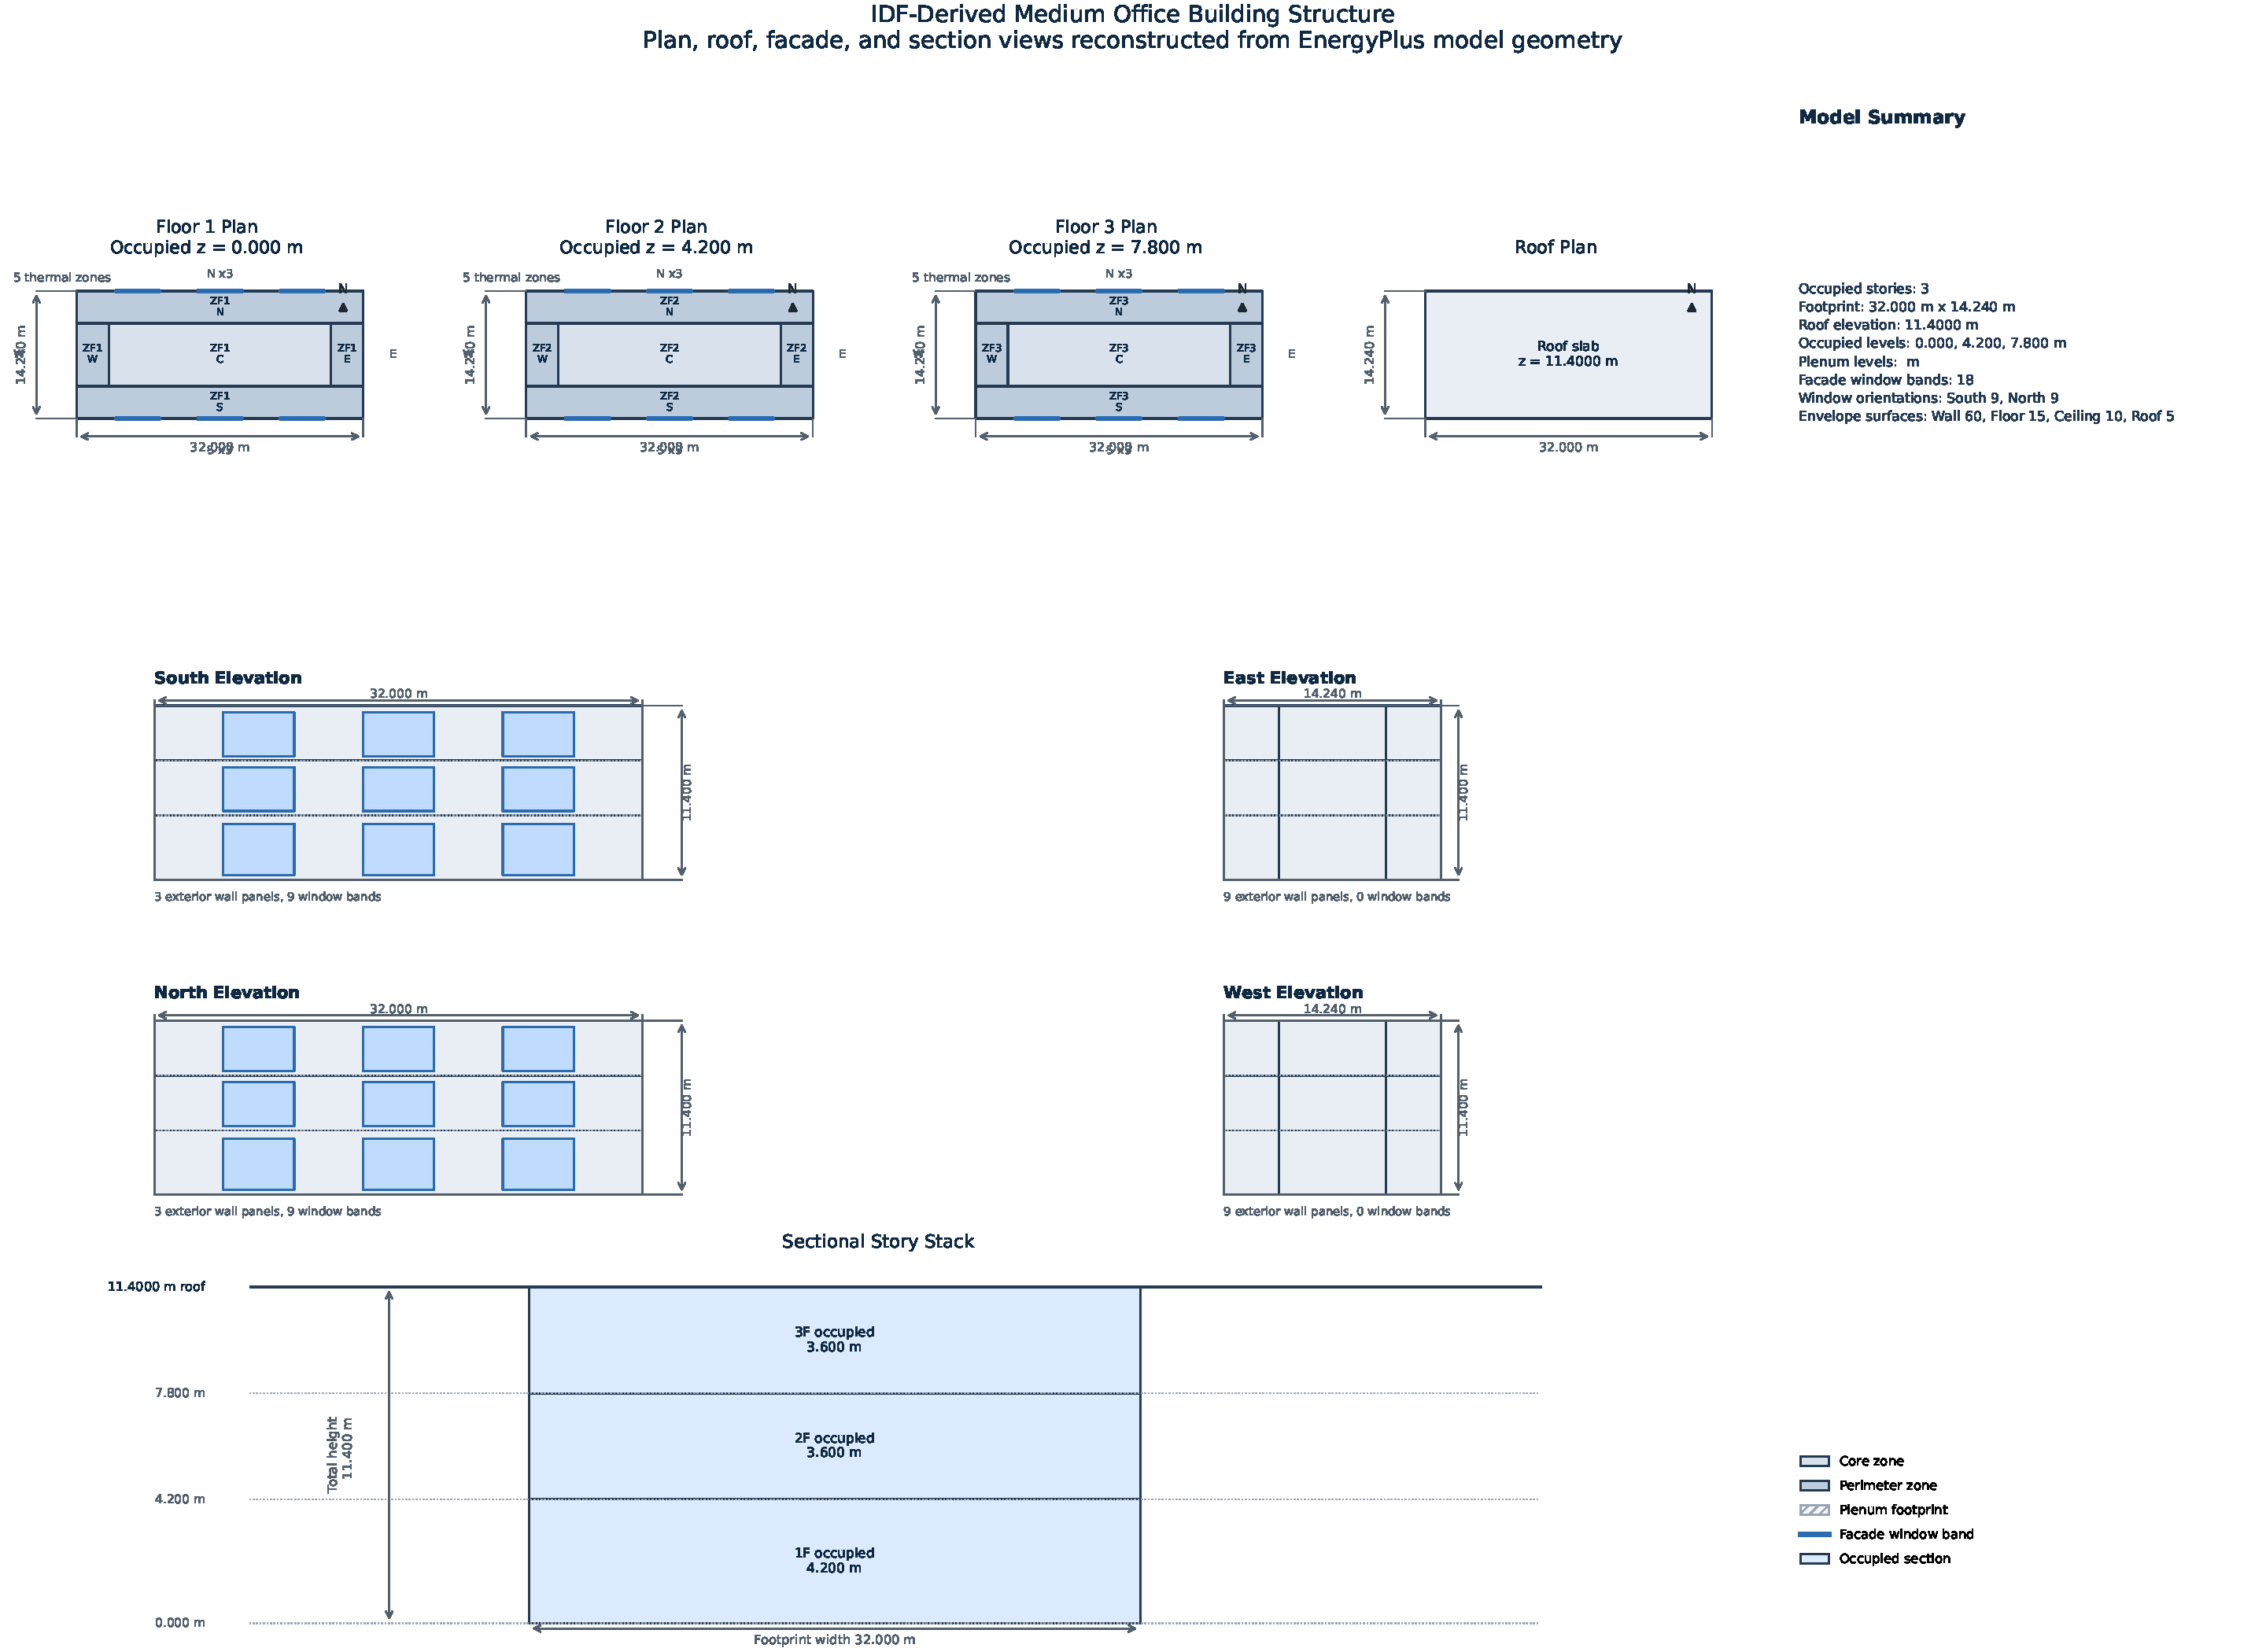
\includegraphics[width=0.90\textwidth,height=0.76\textheight,keepaspectratio]{medium_office_building_model_structure.pdf}

\vspace{0.3em}
\small
该图展示了共享办公建筑母版的各层平面、屋顶平面、四向立面与剖面。五个城市在当前阶段共用这一建筑骨架，以保证比较公平。
\end{frame}

\begin{frame}{两类空调方案设置}
\small
\begin{columns}[T]
    \begin{column}{0.48\textwidth}
        \begin{block}{VRF+DOAS}
            \begin{itemize}
                \item 变制冷剂流量系统
                \item 配独立新风系统
                \item 室外机集中布置
                \item 末端按热分区服务
            \end{itemize}
        \end{block}
    \end{column}
    \begin{column}{0.48\textwidth}
        \begin{block}{FCU+DOAS}
            \begin{itemize}
                \item 风机盘管末端
                \item 配独立新风系统
                \item 含冷热水系统
                \item 由冷源与热源共同支撑
            \end{itemize}
        \end{block}
    \end{column}
\end{columns}

\vspace{0.4em}
\begin{alertblock}{统一比较前提}
两类系统的服务分区数量相同，当前均为 \ctextbf{15 个分区}；设计新风量保持一致，为 \ctextbf{\SI{3.35185}{\meter^3\per\second}}。
\end{alertblock}
\end{frame}

\begin{frame}{系统平面表达与建筑挂接}
\small
\begin{columns}[T]
    \begin{column}{0.49\textwidth}
        \centering
        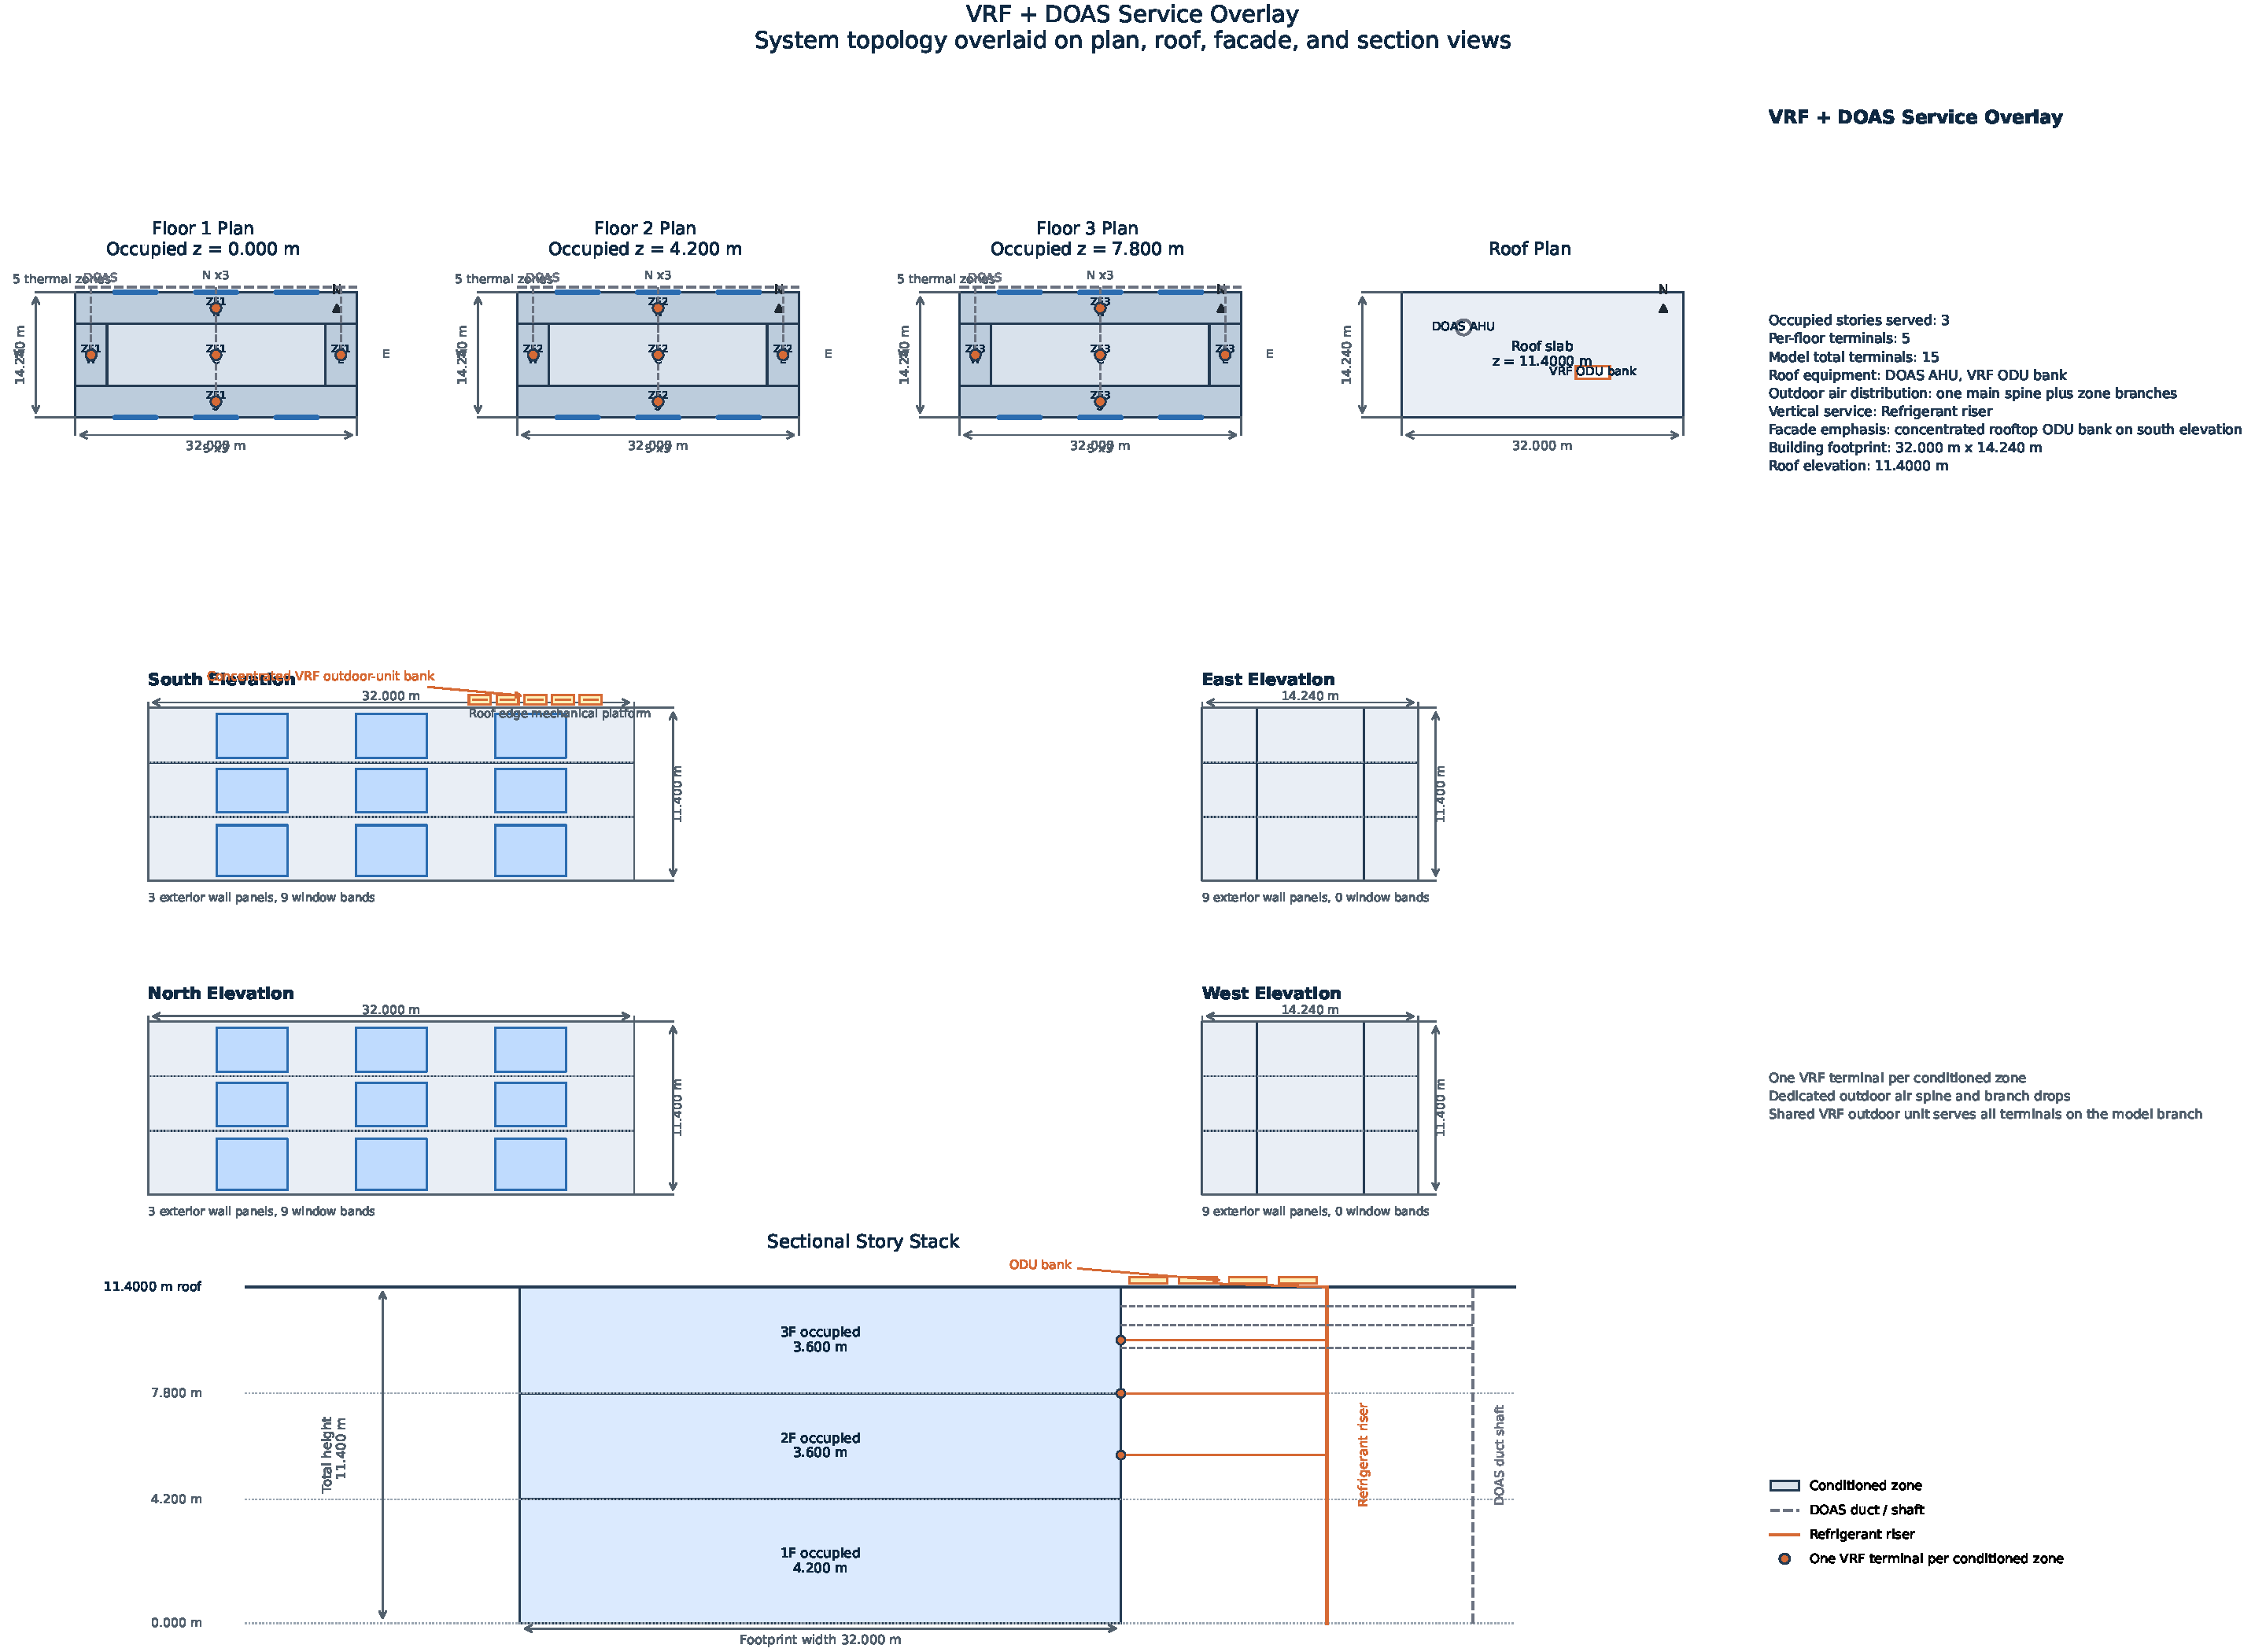
\includegraphics[width=\textwidth,height=0.62\textheight,keepaspectratio]{medium_office_typical_floor_vrf_doas.pdf}

        \vspace{0.2em}
        \textbf{VRF+DOAS}
    \end{column}
    \begin{column}{0.49\textwidth}
        \centering
        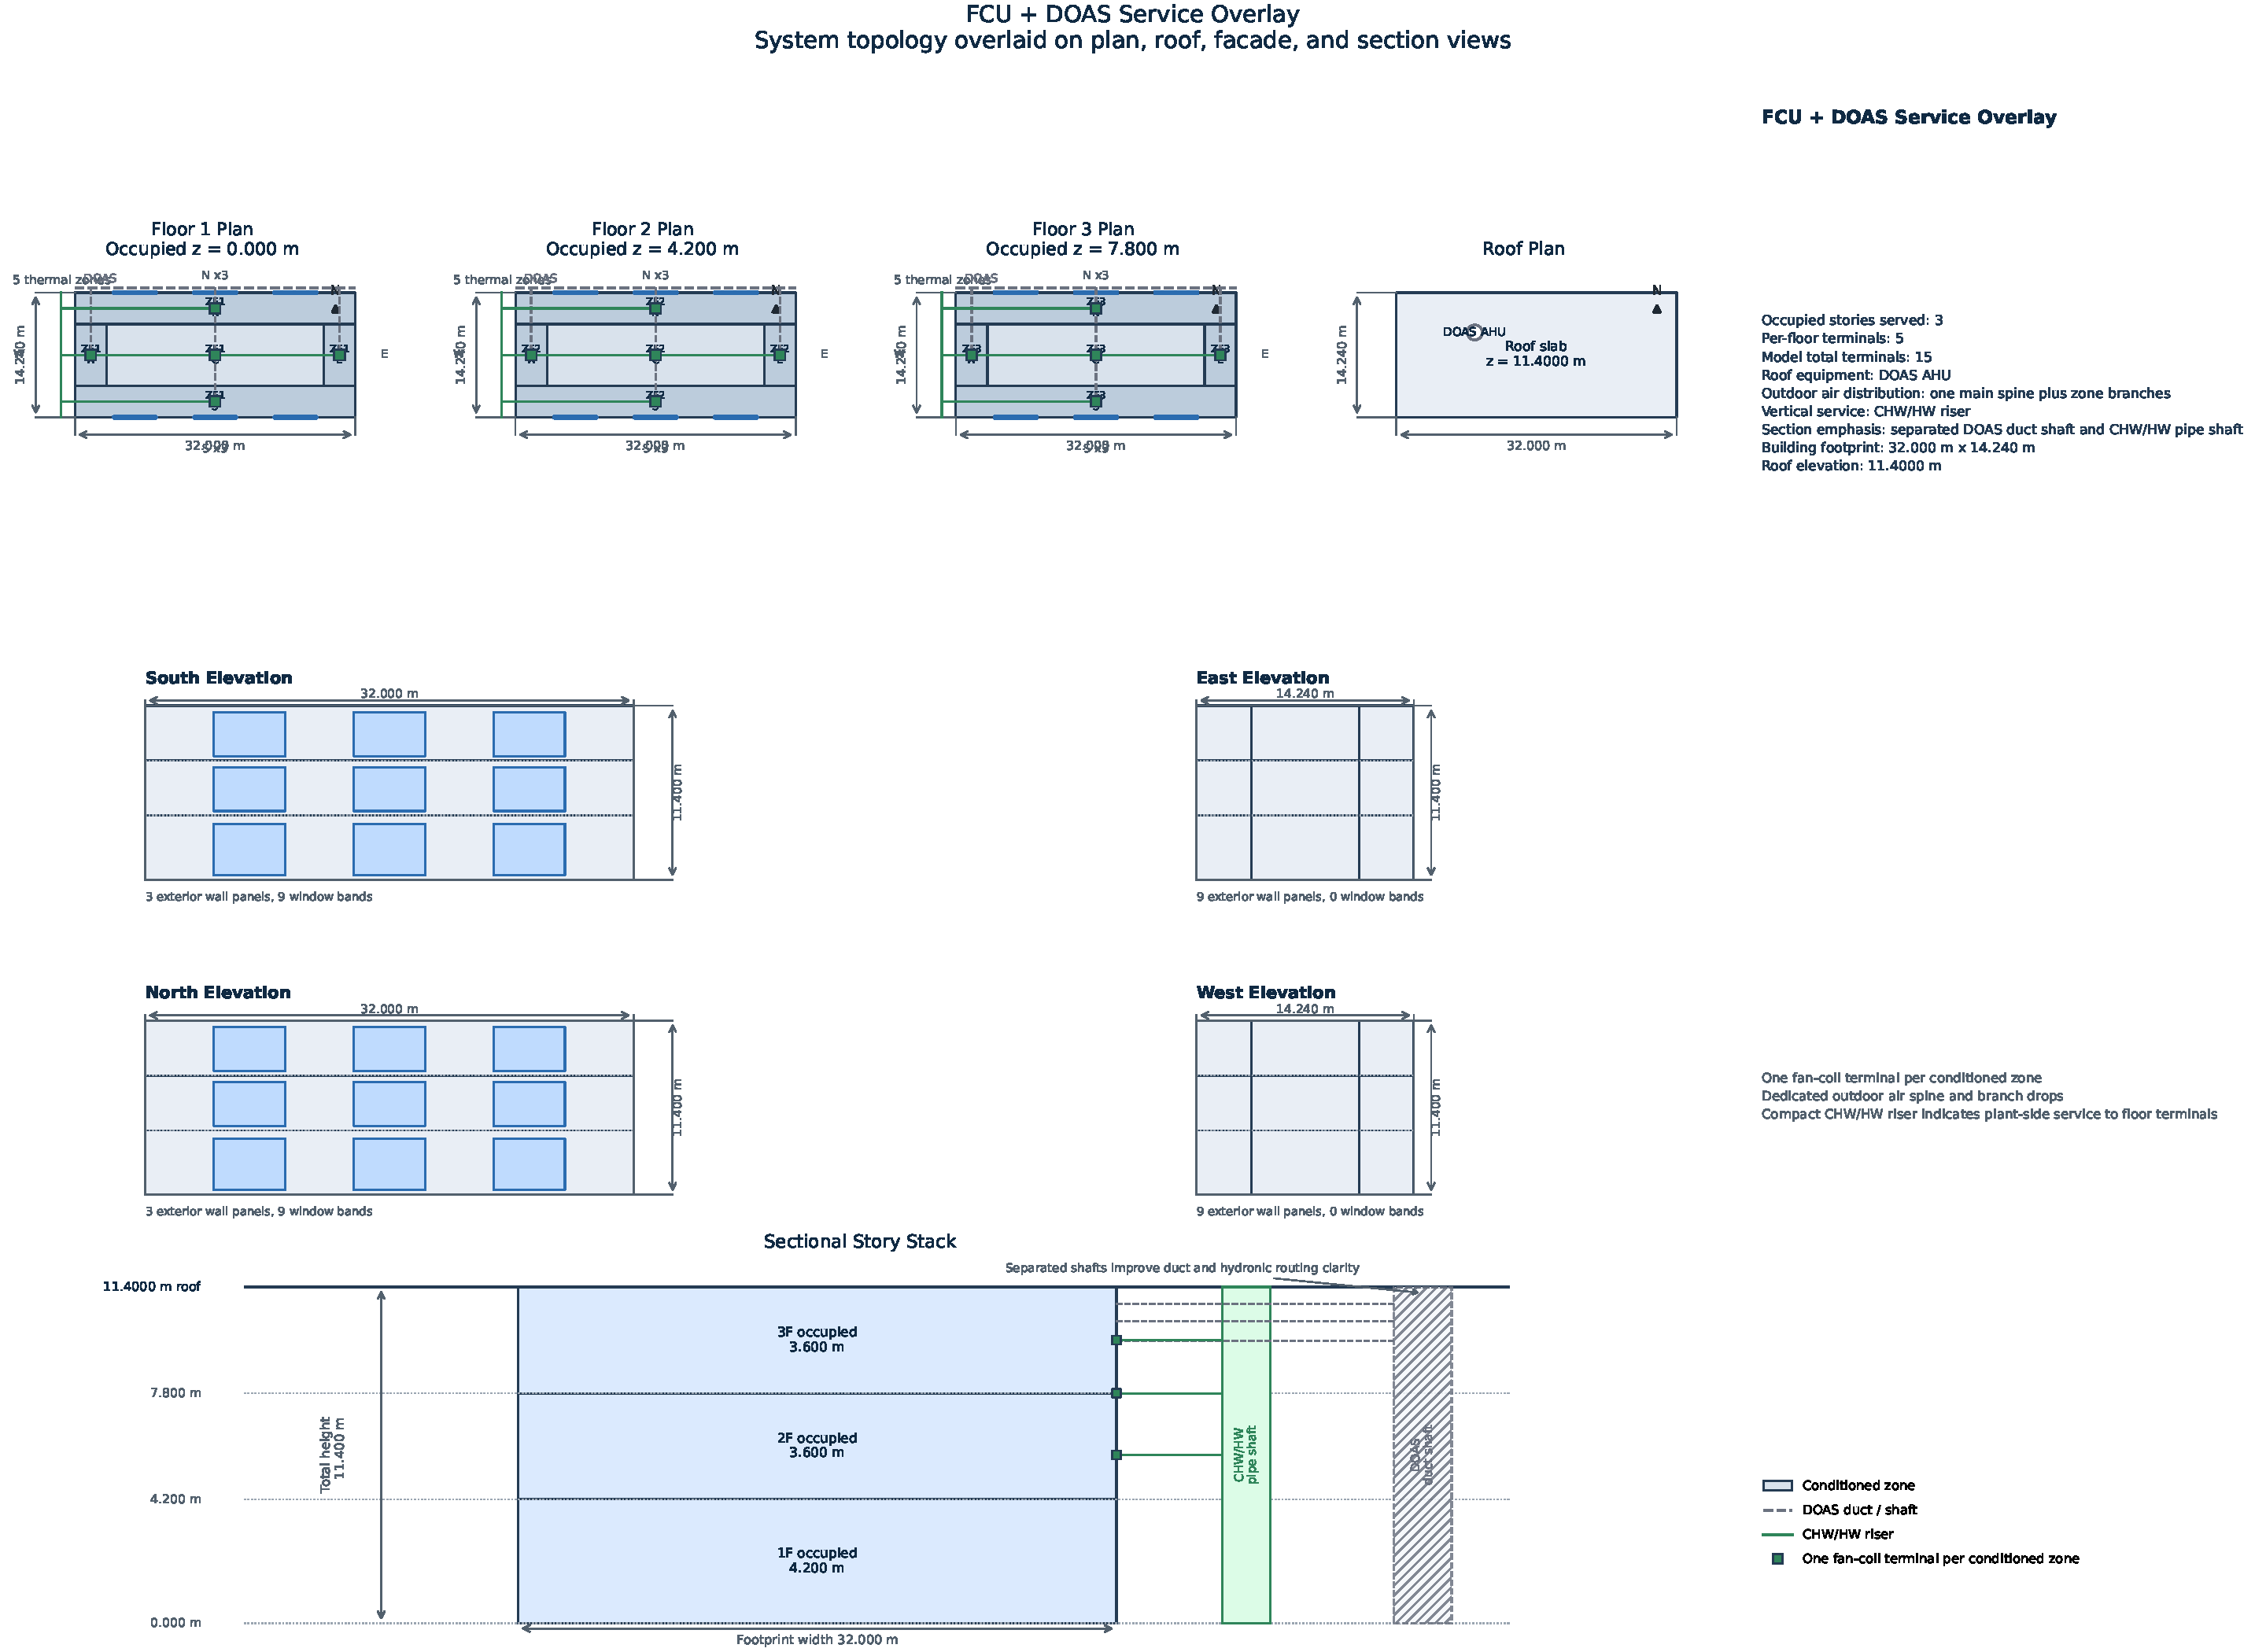
\includegraphics[width=\textwidth,height=0.62\textheight,keepaspectratio]{medium_office_typical_floor_fcu_doas.pdf}

        \vspace{0.2em}
        \textbf{FCU+DOAS}
    \end{column}
\end{columns}

\vspace{0.3em}
\small
两类方案均基于同一办公楼平面展开，但末端组织、管线表达与设备挂接方式不同，这为后续适宜性评价提供了统一而可比的建筑载体。
\end{frame}

\begin{frame}{指标体系与评价逻辑}
\small
\begin{columns}[T]
    \begin{column}{0.32\textwidth}
        \begin{block}{负荷指标}
            \begin{itemize}
                \item 峰值冷负荷
                \item 峰值冷负荷密度
                \item 年冷负荷
                \item 年热负荷
            \end{itemize}
        \end{block}
    \end{column}
    \begin{column}{0.32\textwidth}
        \begin{block}{运行指标}
            \begin{itemize}
                \item 年空调电耗
                \item 单位面积空调电耗
                \item 城市间系统差异
            \end{itemize}
        \end{block}
    \end{column}
    \begin{column}{0.32\textwidth}
        \begin{block}{设备指标}
            \begin{itemize}
                \item 设计冷量
                \item 终端数量
                \item 新风量边界
            \end{itemize}
        \end{block}
    \end{column}
\end{columns}

\vspace{0.4em}
\begin{alertblock}{评价边界}
当前 \texttt{FCU+DOAS} 仅统计空调电耗，\ctextbf{尚未纳入锅炉燃料消耗}，因此不能直接据此下综合能耗最终结论。
\end{alertblock}
\end{frame}

\section{结果与结论}

\begin{frame}{理想负荷层的关键结论}
\small
\begin{itemize}
    \item 深圳峰值冷负荷最高，为 \ctextbf{\SI{327.092}{\kilo\watt}}，说明制冷需求最强。
    \item 沈阳年热负荷最高，为 \ctextbf{\SI{454752.566}{\kilo\watt\hour}}，反映北方供热需求显著。
    \item 成都年总理想负荷强度最低，为 \ctextbf{\SI{133.344}{\kilo\watt\hour\per\square\meter}}。
    \item 重庆峰值冷负荷为 \ctextbf{\SI{296.424}{\kilo\watt}}，年总理想负荷强度为 \ctextbf{\SI{150.137}{\kilo\watt\hour\per\square\meter}}。
    \item 重庆整体表现介于成都与天津之间，说明同属夏热冬冷地区的城市之间仍存在差异。
\end{itemize}
\end{frame}

\begin{frame}{峰值冷负荷密度对比}
\centering
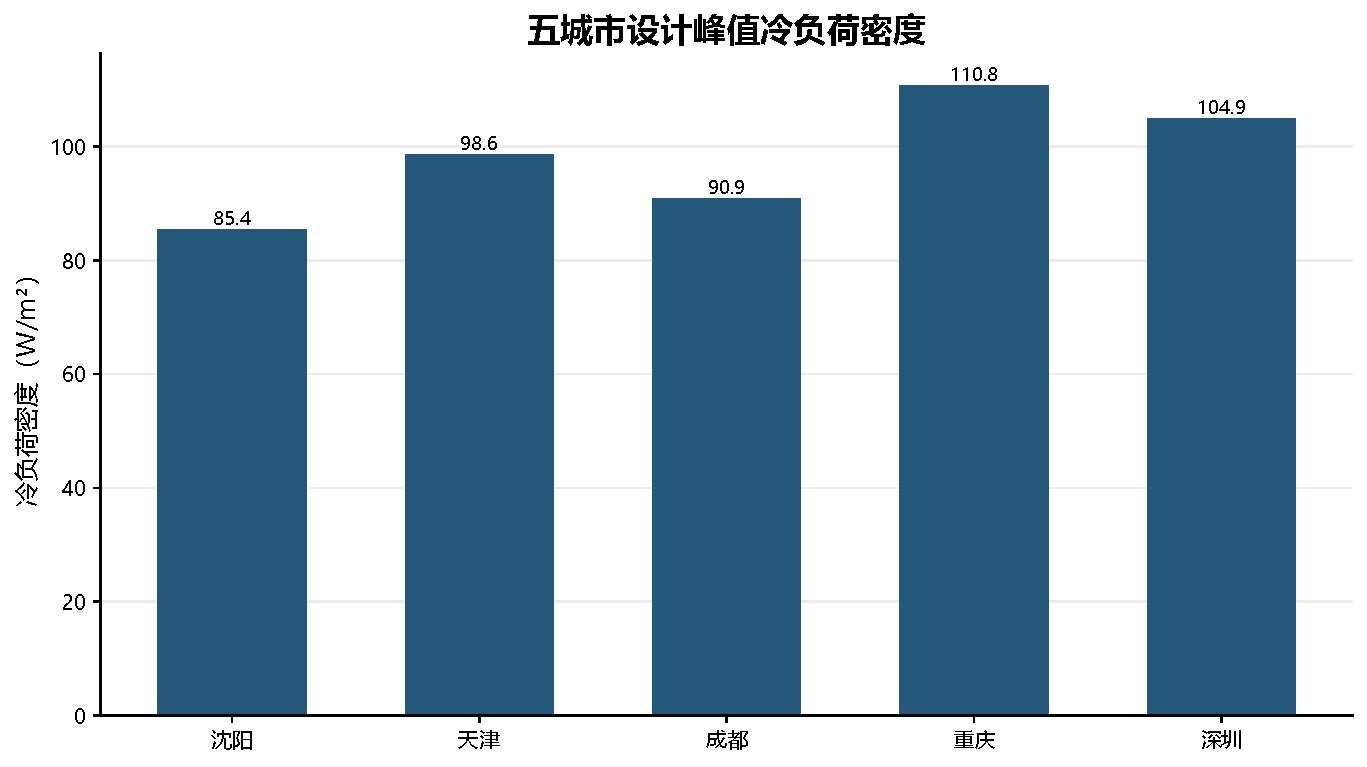
\includegraphics[width=0.9\textwidth,height=0.72\textheight,keepaspectratio]{peak_cooling_load_density_by_city.pdf}

\vspace{0.4em}
\small
深圳峰值冷负荷密度最高，达到 \SI{65.655}{\watt\per\square\meter}；重庆为 \SI{59.499}{\watt\per\square\meter}，高于成都和天津，但低于深圳。
\end{frame}

\begin{frame}{年冷负荷与年热负荷对比}
\centering
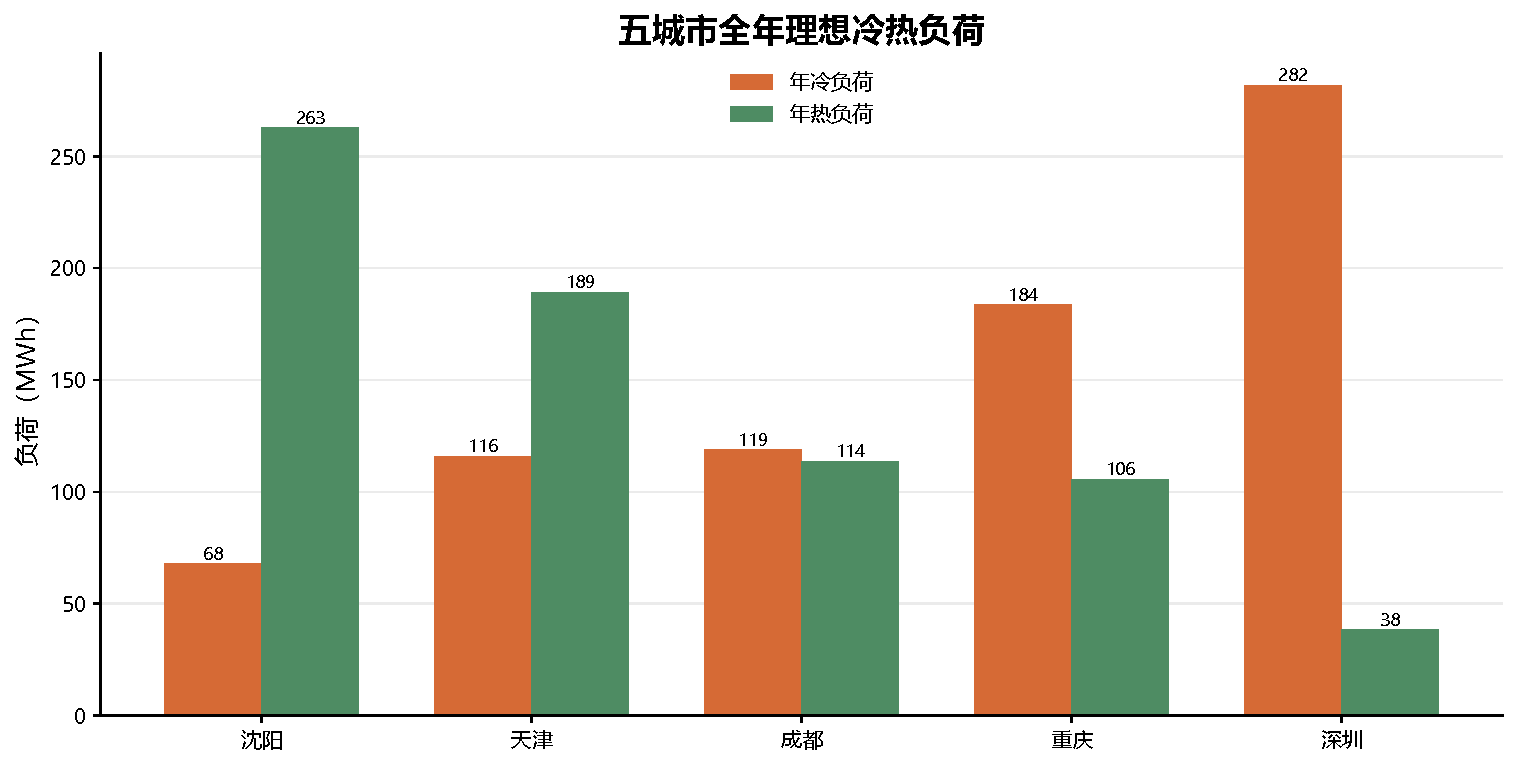
\includegraphics[width=0.92\textwidth,height=0.72\textheight,keepaspectratio]{annual_ideal_loads_by_city.pdf}

\vspace{0.4em}
\small
该图体现了五个城市全年冷热需求构成的差异。沈阳供热占比最突出，深圳全年明显以制冷为主，重庆则补充了夏热冬冷地区样本的中间层次。
\end{frame}

\begin{frame}{系统空调电耗强度对比}
\centering
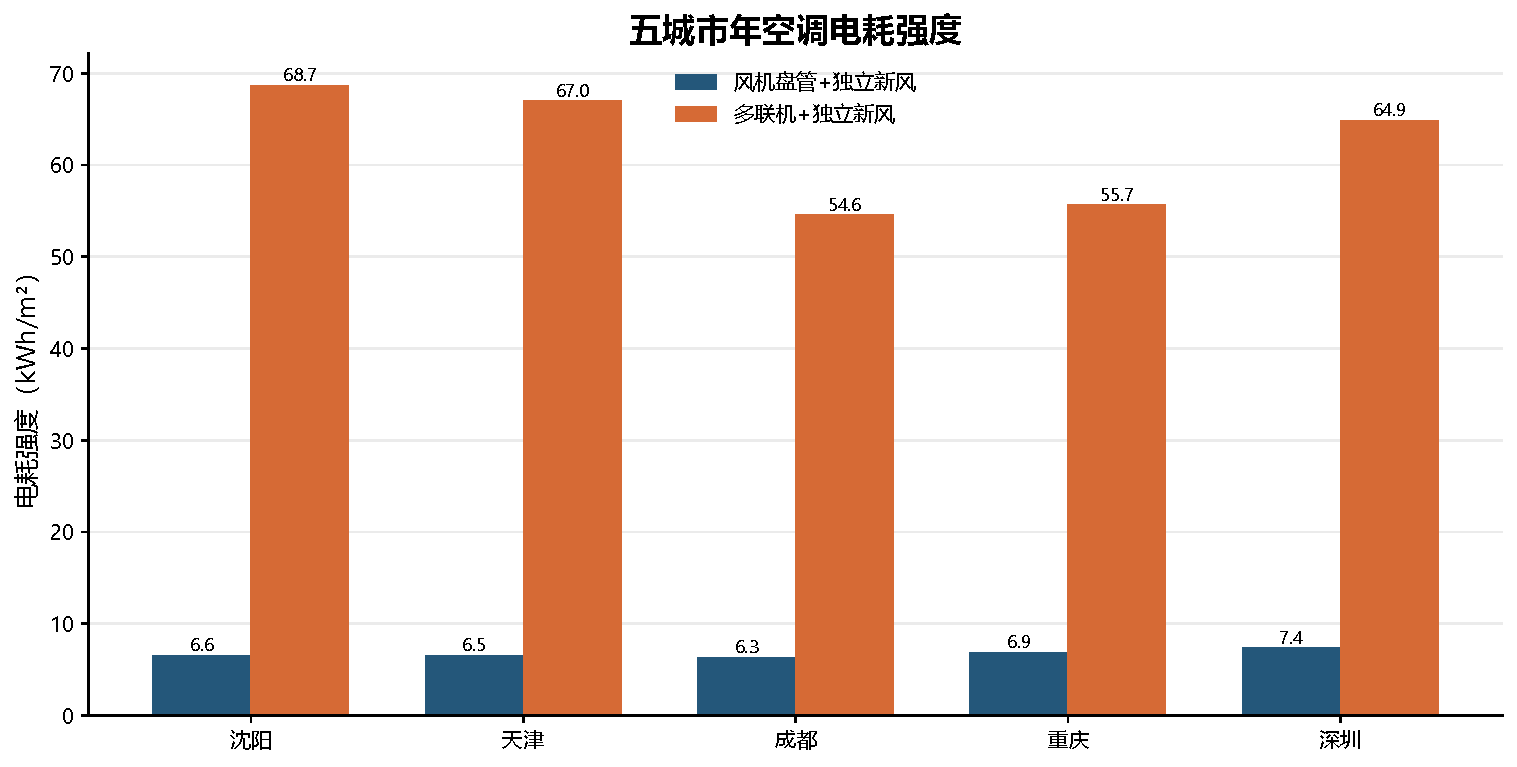
\includegraphics[width=0.92\textwidth,height=0.72\textheight,keepaspectratio]{system_electricity_per_m2_by_city.pdf}

\vspace{0.4em}
\small
\texttt{VRF+DOAS} 的年空调电耗强度范围为 \SIrange{115.174}{173.566}{\kilo\watt\hour\per\square\meter}，\texttt{FCU+DOAS} 为 \SIrange{10.489}{12.367}{\kilo\watt\hour\per\square\meter}。但这里的比较口径仅为空调电耗。
\end{frame}

\begin{frame}{设计冷量对比}
\centering
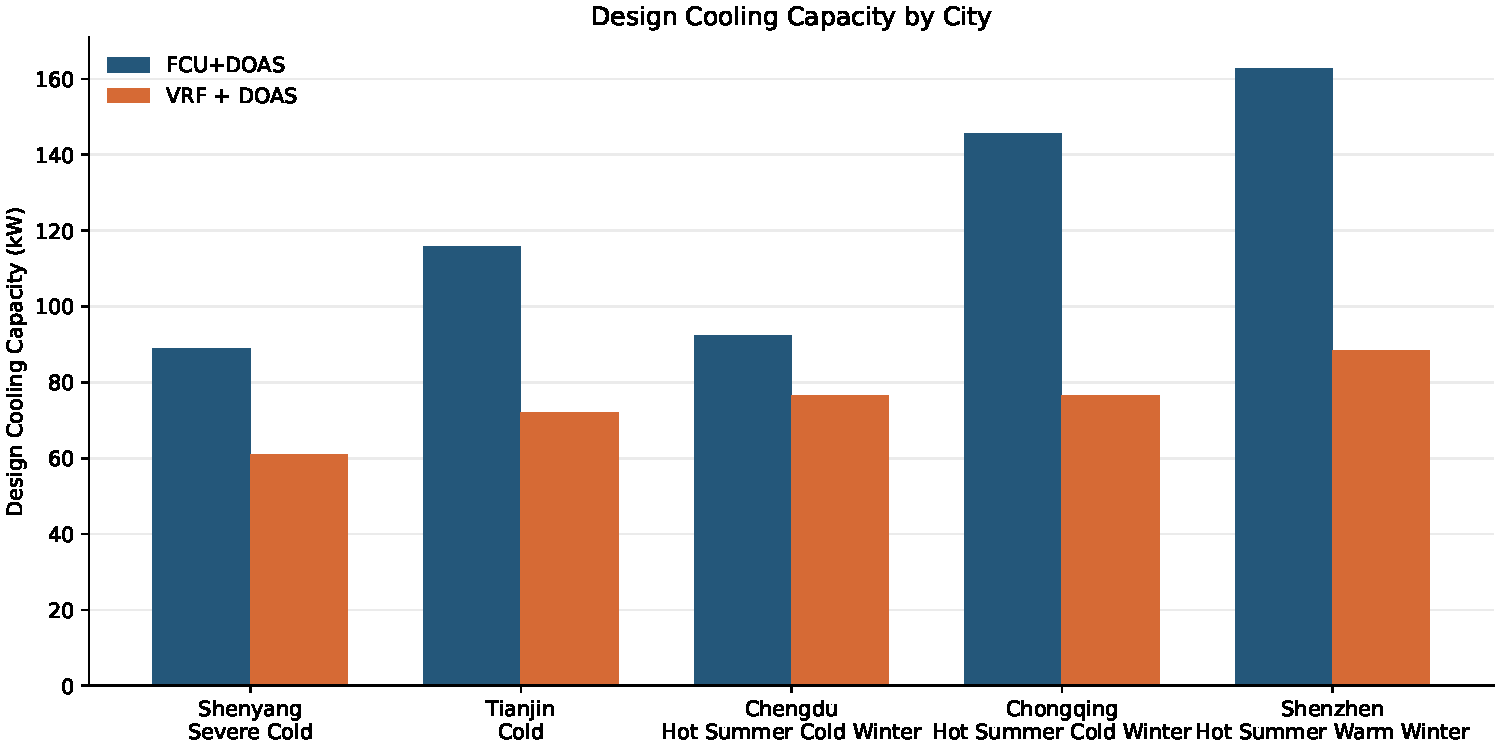
\includegraphics[width=0.92\textwidth,height=0.72\textheight,keepaspectratio]{design_cooling_capacity_by_city.pdf}

\vspace{0.4em}
\small
设计冷量总体随制冷需求增强而增大。最小为沈阳 VRF 的 \SI{464.250}{\kilo\watt}，最大为深圳 FCU 的 \SI{711.085}{\kilo\watt}；重庆位于成都与天津之间。
\end{frame}

\begin{frame}{重庆样本的补充意义与适宜性评价}
\small
\begin{block}{为什么加入重庆}
重庆与成都同属夏热冬冷地区，但其峰值冷负荷、年总理想负荷强度与系统设计冷量都高于成都，说明同一气候分区内部仍有差异，不能简单用单一城市代表整个区域。
\end{block}

\vspace{0.4em}
\begin{itemize}
    \item 北方城市如沈阳、天津，应重点关注\ctextbf{供热侧影响}。
    \item 南方及中西部城市如成都、重庆、深圳，更需要关注\ctextbf{制冷强度与设计冷量}。
    \item 两类系统应保持\ctextbf{并列比较}，不宜在研究开始前预设优劣。
\end{itemize}
\end{frame}

\begin{frame}{结论、局限与展望}
\small
\begin{block}{主要结论}
本文建立了五个城市、15 组工况的统一比较框架，明确了气候分区对负荷和系统表现的显著影响。
\end{block}

\begin{alertblock}{当前局限}
\texttt{FCU+DOAS} 尚未纳入锅炉燃料消耗，且五个城市当前仍采用统一围护结构，因此本文更适合作为\ctextbf{阶段性方案筛选与方法比较成果}。
\end{alertblock}

\begin{exampleblock}{后续工作}
后续可进一步引入分区化围护结构参数、补齐全口径能耗，并扩展到碳排放与控制策略评价。
\end{exampleblock}
\end{frame}

\QApage

\end{document}
